% !TEX root = ../thesis.tex

\chapter{Analytical part}
\label{sec:analytical}
\section{Problem description} \label{sec:description}
Most important thing for each e-commerce project is to predict behavior of their customers or visitors.
In that complex prediction statistics methods are little bit problematic, because of they don't calculate with most of psychology
and sociology aspects.
From statistic methods we can get some basic framework of our prediction income, but in many cases the reality
of the products life can be really different and can crash company business model.
So we are trying to find complex models to predict company income to reflect business plan.
The best approach is the create business plans with that modeling before, so we can minimize the risk of our business.
Two phenomena of particular interest for assessing modelling options are the~\ref{subsec:decoy} and~\ref{subsec:lock-in} principles.
As is written in~\cite{patel}, this modelling is especially used when  the new brand or product is established.
But not in stores on daily basis.
This is caused by the research cost for that studies.\\
\\
\textbf{Decoy effect} \label{subsec:decoy}\\
The Decoy Effect or the Asymmetric Dominance Effect is a cognitive bias in which consumers will tend to have a specific
change in preferences between two vendor options when also presented with a third option that is asymmetrically dominated.
Simply put when there is a third strategically important choice, aka the decoy, then the consumer is more likely to
choose the more expensive of the other two options.
An option is asymmetrically dominated when it is inferior in all respects to one option.
However, in comparison to the other option, it is inferior in some respects and superior in others.
In other words, it is completely dominated by one option and only partially dominated by the other.
When the asymmetrically dominated option is present, a higher percentage of consumers will prefer the dominating
option than when the asymmetrically dominated option is absent.
The asymmetrically dominated option is therefore a decoy serving to increase preference for the dominating option.\\
\\
\textbf{Lock-in} \label{subsec:lock-in}\\
Proprietary lock-in, or customer lock, makes the customer dependent on the products and services of a particular
entity by creating significant costs of switching to the products and services of others.
This can be achieved, for example, by the use of non-standardized patented product components.
Locking, which creates barriers to market entry, can be avoided by antitrust measures.
Proprietary locking is for example blocking mobile phones for only one of the operators or DRM.

\section{Mathematical Background and Marketing introduction} \label{sec:introduction}
Overview of mathematical equation and approaches used to my prediction in context of Marketing approaches usually used to predict customer behavior.\\
\subsection{Models} \label{subsec:models}
\textbf{Simple Dynamic Models} \label{subsec:simpleDynamicModels}\\
One of the simplest models that have been considered for human behavior modeling are dynamic single prices,

\begin{equation} \label{eq:1}
X_k = f(x_k, t) + \xi(t)
\end{equation}
\\
where the function $f$ is dynamic evolution of vector $Xk$ at time $k$.
Than we can define an observation process like

\begin{equation} \label{eq:2}
Y_k = h(X_k, t) + \eta(t)
\end{equation}
\\
\textbf{Multiple Dynamic Models} \label{subsec:multipleDynamicModels}\\
Human behavior is usually not as simple as a single dynamic model.
For complex model of human behavior we can use some alternatives.
In many case we have to use different models for each person's dynamic response~\cite{wilsky}.
Than we can test each instance of response to predict person's state.
From that we can established multiple model approach to predict future values of state variables.
In this situations is Kalman's filter calculation very usefully for realtime application because of it's sufficiently small costs of resources.
This approach breaks the person's overall behavior down into several prototypical behaviors.~\cite{pantland}
Mathematically, this is accomplished by setting up a set of states $S$, each associated with a Kalman's filter and a particular dynamic model.\\
\\
\textbf{A linear ODE model} \label{subsec:ode}\\
In this model the strength of flux between brands or products are determined by perceived brand quality,
based upon binary comparisons.
The simplest response to such comparisons is an attempt by customers to minimize the expected regret resulting
from any choice, which is what is assumed here.
It has previously been shown that the choice rule recognizes the attribute-wise proximity of an alternative
to other brands, and it is therefore appropriate for preference change to be modelled on the pair-wise ranking
of brands in each quality, the simplest perhaps being to assign a positive score to a brand for each successful comparison.
Thus customers attempt to minimize their anticipated regret by opting – on any particular quality – for the safe bet.
More sophisticated customer behavior, capable of not only ranking brands but discriminating according to the size of proximity gap
requires more complex modelling, but may be justified since it appears that subjective attribute valuations at least are nonlinear,
reference-point-dependent functions.\\
\\
\textbf{Discrete-time model} \label{subsec:discrete}\\
Discrete models or difference equations \footnote{Difference equations can be viewed either as a discrete analogue of differential equations, or independently.
They are used for approximation of differential operators, for solving mathematical problems with recurrences, for building various discrete
models, etc.} are used to describe biological events or whole systems for which is natural to regret time at fixed discrete intervals.

\begin{equation} \label{eq:4}
\hat{X}_{k}^{(i)} = X_{k}^{*(i)} + K_k^{(i)}(Y_k - h^{(i)}(X_{k}^{*(i)},t))
\end{equation}
\\
where the superscript $(i)$ denotes the $i$th Kalman's fillter.
The measurement innovations process for the ith model.

\begin{equation} \label{eq:5}
\Gamma_k^{(i)}= Y_k - h^{(i)}(X_k^{*(i)}), t)
\end{equation}
\\
The measurement innovations process is zero-mean with covariance $R$.
The ith measurement innovations process is, intuitively, the part of the observation data that is unexplained by the ith model.
The model that explains the largest portion of the observations is, of course, the model most likely to be correct.
Thus, at each time step, we calculate the probability $Pr^{(i)}$ of the m-dimensional observations $Y_k$ given the $i$th model's dynamics
\\
\begin{equation} \label{eq:6}
Pr^{(i)}(Y_k|X_k^*) = \frac{exp(-\frac{1}{2}\Gamma_k^{(i)T}R^{-1}\Gamma_k^{(i)}}{(2\pi)^{m/2} Det(R)^{1/2}}
\end{equation}
\\
and choose the model with the largest probability.
This model is then used to estimate the current value of the state variables, predict their future values, and choose among alternative responses.

\subsection{Modeling and Prediction of Human Behavior} \label{subsec:prediction}

We have an observations Y as a function h of the state vector and time.
Both $\xi$ and $\eta$ are processes with known density matrices.
Using Kalman's result, we can then find optimal linear estimate $X_k$ using th Kalman's filter \footnote{In statistics
and control theory, Kalman filtering, also known as linear quadratic estimation (LQE), is an algorithm that
uses a series of measurements observed over time, containing statistical noise and other inaccuracies, and produces
estimates of unknown variables that tend to be more accurate than those based on a single measurement alone, by estimating
a joint probability distribution over the variables for each timeframe.
The filter is named after Rudolf E. Kálmán, one of the primary developers of its theory.}

\begin{equation} \label{eq:3}
X = X_{k}^{*} + K_x(Y_k - h(X_{k}^{*},t))
\end{equation}
\\
provided that the Kalman gain matrix $Kk$ is chosen correctly~\cite{kalman}.
This method iterates for each step $k$ and the filter algorithm use a state prediction at each time step $k$,
the filter algorithm uses a state prediction $X$, an error covariance matrix prediction $P_k^*$,
and a sensor measurement $Y_k$ to determine an optimal linear state estimate $X$.
If we want to predict human's future state whe can use this mechanism with larger time steps.
This mechanism is used e.g. in a car, such a prediction capability can allow us to maintain synchrony with the driver.
In experience of Alex Pentland work \footnote{MIT's Human Dynamics Laboratory and the MIT Media Lab Entrepreneurship
Program, co-leads the World Economic Forum Big Data and Personal Data initiatives, and is a founding member
of the Advisory Boards for Nissan, Motorola Mobility, Telefonica, and a variety of start-up firms.}, this type of prediction
is useful only for short time periods, for instance, in the case of quick hand motions for up to one-tenth of a second.
Especially $f$, $h$ are linear functions and $\xi$, $\eta$ are gaussian.
This functions are commonly extended to "well-behaved" nonlinear problems by approximating the nonlinear system by linear functions
using a local Taylor expansion \footnote{Taylor series is a representation of a function as an infinite sum of terms that are calculated from
the values of the function's derivatives at a single point.}.

\subsection{Specification in customer behavior} \label{subsec:specification}
Customer products such as shampoo or tomato sauce are designed to appeal to customers, encouraging them to buy those products.
It depends on the industry section but all of that designs trying to focus to customer's subconscious.
However, buying behavior is not only a function of the product.
In many cases is the connection of many other functions like a social environment of other customers, the competing
products in the marketplace, brand marketing strategy, seller trust and professionalism and so on.
In order to design the best product, it is necessary to understand not just the physics and chemistry of the product,
but also the psychology of customers and the sociology of customer groups or networks.\cite{patel}

From that paragraphs is see that the general human behavior model has many input variables to represent many kind
of situation to be successfully in future prediction.
Good model in store industry have to be able to learn from actual customer's behavior for each seller and learn
from these datasets in a macroscopic, averaged way.
Alternatively, one can look at individual customers and their buying behavior, and try to derive observable large scale effects.
Ideally it can be predict behavior for each customer and from these results create a global results for each store or industry.\\
\\
\textbf{Loyalty} \label{subsec:loyalty}\\
Loyalty is the tendency for some customers to use the same products or brands again.
This behavior we can describe with a systems of ordinary differential equations.
The stronger the loyalty, the slower the changes in numbers of people buying particular products.
For discrete-time models, the degree of loyalty corresponds to the size of diagonal elements in a transition matrix.
In the modelling we have to calculate with the no loyalty model too.
In some industry like a supermarkets, peoples buy from other reason so some of our input variables in modelling should be
detection of loyalty in out industry.
Next aspect of loyalty would be a memory effect, to represent people returning to products they had previously used,
after trying something new they then did not like.
This could be taken into account perhaps by using recurrence relations or differential equations of higher than first order or even employing
delay-differential equations.\\
\\
\textbf{Sociology} \label{subsec:sociology}\\
Mean sociology in this context as how peoples buying are influenced each other.
With some kind of trends to buy the same brands or products.
There is an option from lock-in~\ref{subsec:lock-in}, with one product dominating the market.
This option is very hard to relevant test, because of the data of huge companies which dominates some kind
of industry are very hard to legally get.
Even if theirs competitors have more or less identical products.
This effect and its opposite, are easily modelled by ODE~\ref{subsec:ode} and discrete-time models.
Opposite is very important in sociology because of people wanting to be different sometimes from irrationals reasons.

\subsection{Markov Chains} \label{subsec:chain}
A Markov chain is a process that occurs in a series of time-steps in each of which a random choice is made
among a finite (or also enumerable) number of states; since both the index set and the state space are discrete,
we denote by $X_n≡X(t_n)$ the transition probability can then be represented by a matrix $P=(p_{ij})$, where pij is
the probability of moving from state i to state j: $p_{ij}=Prob[X_{n+1}=j|X_n=i]$. For homogeneous chains, these
probabilities do not depend on t, i.e., they are stationary. Then, the initial distribution, together with the
transition matrix $P$, determines the probability distribution for any state at all future times.\\
\begin{figure}[h!]
	\begin{center}
		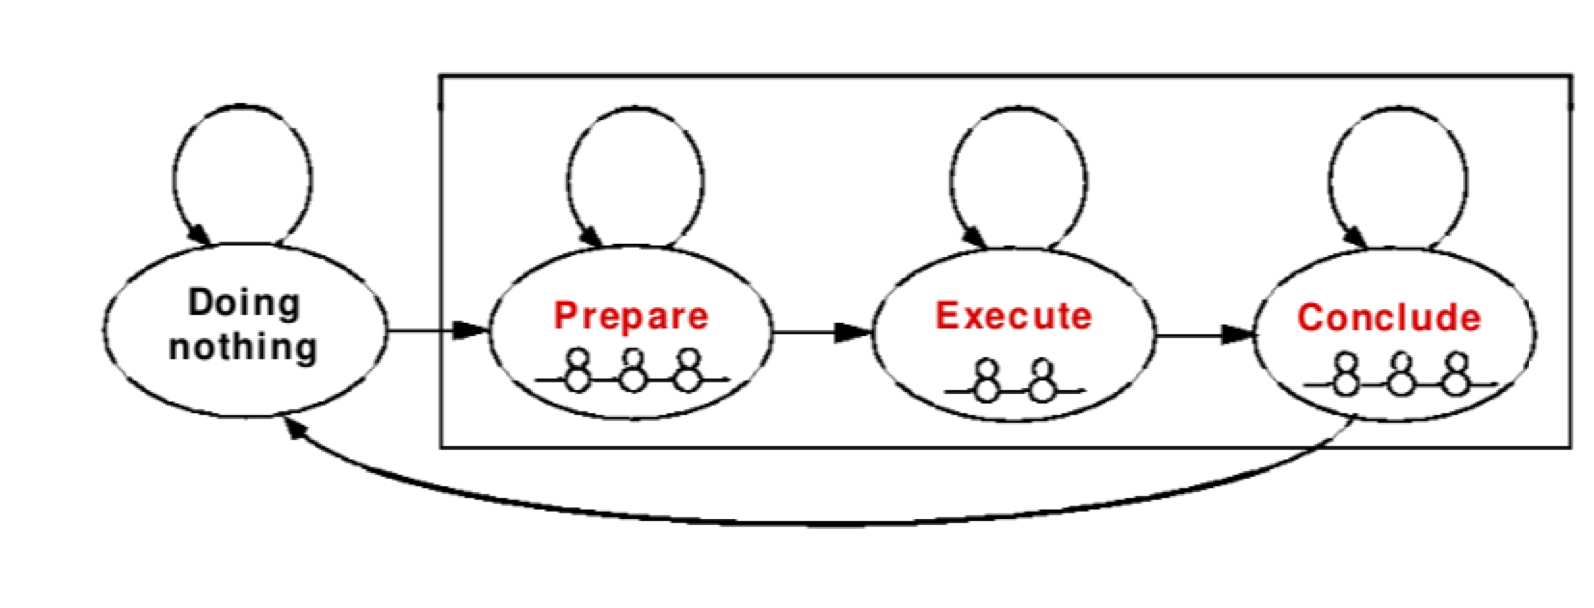
\includegraphics[width=140mm]{markov_model.png}
	\end{center}
	\caption{Basic schema of Markov model in human decision}
	\label{Markov model}
\end{figure}
\\
\textbf{A Markov model with social influences} \label{subsec:markov}\\
This model is based on Markov chains (Markov chain description), better than the time continues differential
equations which are especially use.
To use that model approach we first have to develop the possibility of a decoy effect.
Then we introduce sociology and obtain results for lock-in analogous.
These Markov models display both important similarities to and differences from the previous models, and may be simpler to work with.
The last but not least pros of that models is very good graphical representation.\\
\\
\textbf{An Experiment Using Markov Dynamic Models} \label{subsec:markov_dynamic}\\
Shopping is natural-feeling and familiar type of human behavior that exhibits complex patterns that last from several
seconds to many days.
These characteristics make shopping little bit nearly ideal experimental for modeling human behaviors.
In the case of shopping, the macroscopic actions are events like needs, choosing brands, choosing seller.
The internal states are the individual steps that make up the action, and the observed variables will be changes during the shopping process
workflow in which can be customer decision changed.
The intuition is occasionally important, but this belongs to special market and marketing persons identification such
a buying shoes by a single woman in production age.\\
\\
\textbf{Modeling and Prediction of Human Behavior may consist of the following steps:}\\
\begin{enumerate}
	\item needs decision make
	\item looking across the site to find some adequate
	\item make action decision
	\item shopping workflow process in selected site
	\item make final payment
\end{enumerate}
\\
Psychology covers what, and how, aspects of the actual items on the shelves influence people to make their choices,
possibly buying something different from previously.
Advertising might be comprise into these characteristics but could also possibly be considered as part of the sociological
influences (point 1 and 2), especially if the advertising takes the form of a well known figure endorsing a product.
More specifically, the following four properties have been identified by Unilever Research~\cite{patel} as being important
and their influences were included in one or more models:

\begin{enumerate}
	\item Minimise anticipated regret.
	This refers to how just two products compare with each other as regards different qualities, which can include
	price (or 'affordability' = 1/price).
	A customer might judge one item to be superior to another in all respects.
	The first is then a safe choice for the customer.
	\item Attribute change.
	The introduction of a new product onto the market can change the way customers, or at least some of them, view established brands.
	This might be by drawing attention to some quality which was not previously much regarded, or it might make people give different
	weightings to the (established) qualities when making their decisions.
	The former can be considered to be a special case of the latter.
	\item Outlier avoidance.
	When a number of products are in many aspects quite similar, there can be a tendency for people to avoid ‘strange’ ones, like others which
	are substantially different from the majority in price or some other respect.
	Items near the average can be favoured.
	\item Decision process change.
	A straight choice between two items might be relatively easy.
	They can be compared according to price, size etc\. and a decision made.
	With three or more, comparisons might be made between two things at a time, one could be eliminated and then the winner contrasted
	with a third.
\end{enumerate}
\subsection{Viterbi algorithm} \label{subsec:viterbi}
The Viterbi algorithm is a dynamic programming algorithm for finding the most likely sequence of hidden
states called the Viterbi path that results in a sequence of observed events, especially in the
context of Markov information sources and hidden Markov models (HMM)~\ref{Viterbi schema}.
The algorithm has found universal application in decoding the convolutional codes used in
both CDMA and GSM digital cellular, dial-up modems, satellite, deep-space communications, and 802.11 wireless LANs.
It is now also commonly used in speech recognition, speech synthesis, keyword spotting, computational
linguistics, and bioinformatics.
For example, in speech-to-text (speech recognition), the acoustic signal is treated as the observed sequence of events,
and a string of text is considered to be the "hidden cause" of the acoustic signal.
The Viterbi algorithm finds the most likely string of text given the acoustic signal.
Here you can see Viterbi algoritm implementation in Python language: \\
\begin{lstlisting}[language=python]
# probability == p. Tm: the transition matrix. Em: the emission matrix.
function viterbi(O, S, Π, Tm, Em): best_path
  # To hold p. of each state given each observation.
  trellis ← matrix(length(S), length(O))
  # Determine each hidden state's p. at time 0…
  for s in range(length(S)):
    trellis[s, 0] ← Π[s] * Em[s, O[0]]
  # and afterwards, assuming each state's most likely prior state, k.
  for o in range(1, length(O)):
    for s in range(length(S)):
      k ← argmax(k in trellis[k, o-1] * Tm[k, s] * Em[s, o])
      trellis[s, o] ← trellis[k, o-1] * Tm[k, s] * Em[s, o]
  best_path ← list()
  # Backtrack from last observation.
  for o in range(-1, -(length(O)+1), -1):
    # Most likely state at o
    k ← argmax(k in trellis[k, o])
    # is noted for return.
    best_path.insert(0, S[k])
  return best_path
\end{lstlisting}
\begin{figure}[h!]
	\begin{center}
		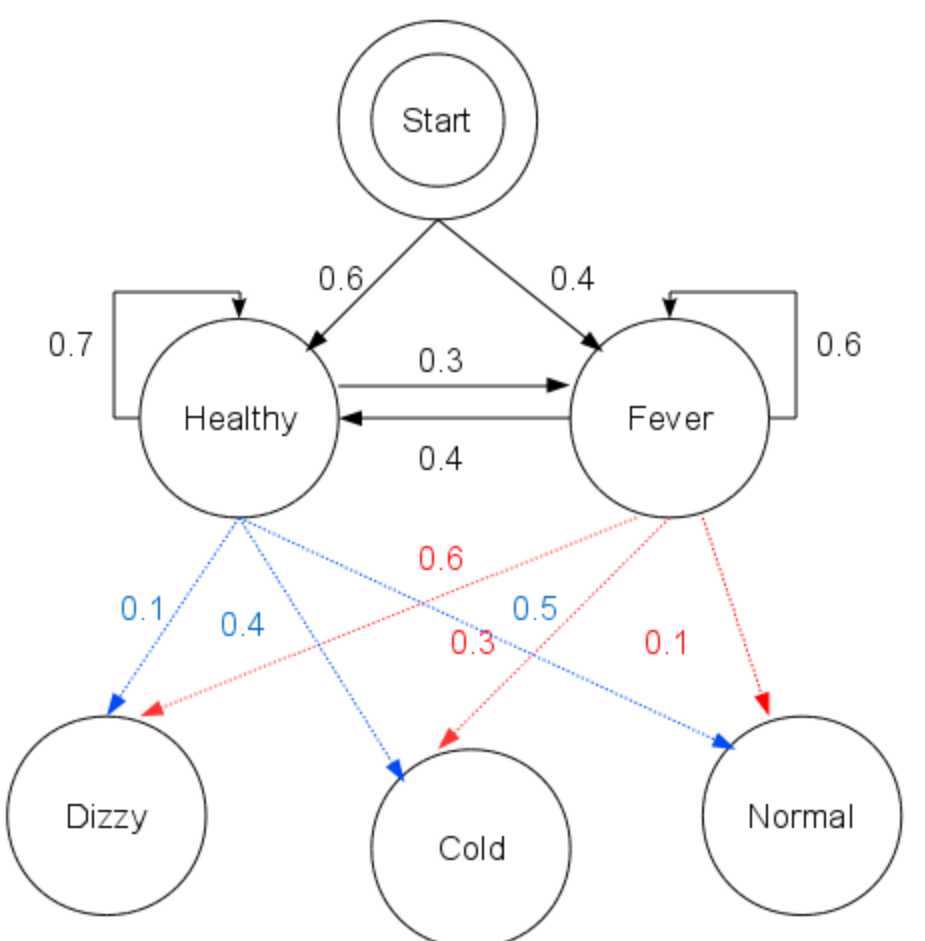
\includegraphics[width=90mm]{viterbi_graph.png}
	\end{center}
	\caption{Viterbi algorithm schema example}
	\label{Viterbi schema}
\end{figure}
\subsection{Predicted effects} \label{subsec:predicted}
\begin{enumerate}
	\item How a decoy product might influence the market.
	The appearance of a third product might remarkably change the market shares of two others, while getting minimal sales itself.
	This effect is one of the most complex biases in customer choice, and has been observed in product classes from chocolate bars
	to electronics to beer.
	The decoy effect illustrates the importance of customer psychology, to understanding how customers recognize products,
	and how customers see quality side to buy the product.

	\item The dynamics of market share is  how sales of products can change during the time.
	For example, even if two products are really equal in all relevant aspects, then after a long time of customer activity it might be that
	each product takes 50\% market share (preserving the symmetry), or one product takes nearly 100\% market share (breaking the symmetry),
	or that there is no steady state, with market dominance alternating between the two brands.
	The second of these three cases is called lock-in, corresponding to one brand obtaining a virtual monopoly,
	which is almost impossible to break.
	From that reason is not legally to create a monopole in some industries and for human purchase behavior is not
	good to calculate with monopole approach.

	\item How a new product will fare, given its quality profile compared with existing brands.
	This question is complementary to that of the decoy, asking what market share a new product will gain rather than how it will
	affect the market shares of existing products.

	\item Choice overload: when there are just too many possible options for potential customers to pick from, and many
	will search the sites without making a purchase.
\end{enumerate}

\subsection{Minimise anticipated regret} \label{subsec:regret}
This modelling property was taken to lead to simple comparisons along the lines of with regard to quality $k$,
is product $i$ better than product $j$?
If the answer to all relevant questions, $k = 1, . . . , nq$, if $nq$ is the number of qualities, is no, then a customer
will not change from $j$ to $i$.
The more times the answer is yes, the faster such a change is likely to happen.
This can be represented by taking the flow-rate constants to be of the form (todo equation)

\section{Customer preferences and decision process} \label{sec:customer_preferences}
Consider a customer whose preference is shared out amongst all the available brands in a market where there are
no empty or zero brands, so that the total of all brands preference shares is 1 (100\%).
The proportion of customer preference held by brand $X$ at time $t$ is denoted by $X(t)$.
For example, if the preference share of brand $A$ is plotted against brand $B$ in a market where only two brands exists,
the point must be somewhere along the straight line $B(t) = 1, A(t)$.
Of interest is the case when a third brand is added, possibly as a decoy.
The additional brand means that the preference distribution changes from being a straight line in the two-dimensional plane $(A, B)$,
to a plane in three-dimensional space $(A,B,C)$.\\
\\
\textbf{Customer decision process} \label{sec:decision}\\
Described in~\cite{patel} show that the standard Logit model~\ref{subsec:logit} for customer choice assumes that
the probability, $p_i$, with which a customer buys a given product $i$ from a range of products $<1, n>$ depends on
the value which customer attaches to that product $V_i$, and the price of the product $P_i$.
This dependence is taken to be of exponential form.
Assuming that guaranteeing that all probabilities are positive)
\\
\begin{equation} \label{eq:7}
p_i = C exp(V_i - P_i)
\end{equation}
\\
where $s$ is a measure of the relative importance of price to the customer, and $C$ is a normalisation constant chosen so that
\\
\begin{equation} \label{eq:8}
\sum_{i=1}^n p_i = 1
\end{equation}
\\
The value $V_i$ is then taken to reflect the influence on the customer of the quality of the product,$Q_i$,
the increased likelihood of the customer buying the same brand as he bought previously (the loyalty effect),
and the peoples who have an influence on a customer (neighbours).
Each of these dependencies are taken to be linear, giving
\\
\begin{equation} \label{eq:9}
V_i = aQ_i + lI_i + hN_i,
\end{equation}
\\
where $I_i$ is an indicator function which is unity if the customer previously bought product i and zero otherwise,
$N_i$ is the number of neighbours who bought product $i$, and $a, l$ and $h$ are constants measuring the relative strength
of each effect.
In such a model the products are all treated independently.
Only coupling between the probabilities occurs through the normalisation constant $C$.
Product $I$ will depend not only on the value and price of that product, $V_i$ and $P_i$, but on the value and prices of all products.
The goal of this section is to formulate a model for this probability which is based on binary comparisons, that is,
on comparisons of two products at a time.\\
\subsection{Logit analysis in marketing} \label{subsec:logit}
Logit analysis is a statistical technique used by marketers to assess the scope of customer acceptance of a product, particularly a new product.
It attempts to determine the intensity or magnitude of customers' purchase intentions and translates that into a measure of actual buying behavior.
Logit analysis assumes that an unmet need in the marketplace has already been detected, and that the product has been designed to meet that need.
The purpose of logit analysis is to quantify the potential sales of that product.
It takes survey data on consumers purchase intentions and converts it into actual purchase probabilities.
Logit analysis defines the functional relationship between stated purchase intentions and preferences, and the actual probability of purchase.
A preference regression is performed on the survey data.
This is then modified with actual historical observations of purchase behavior.
The resultant functional relationship defines purchase probability.

\subsection{Brand or product changing} \label{subsec:brand}
We can mathematically express the process of decision to switch from one brand to another one.
Consider a linear flux $\alpha_{xy}$ of preferences moving to brand $X$ from brand $Y$.
All fluxes have to be strictly positive.
It's in improper to consider negative flux, so really excluded is only zero value.
Flux is the proportion of customer preference to switch to other brand or product from previous one.
In a two brand or two producst market we have these final equations

\begin{equation} \label{eq:10}
\begin{array}{r@{}l}
\frac{dA}{dt} = -\alpha_{BA}A + \alpha_{AB}A \\
\frac{dB}{dt} = +\alpha_{BA}A - \alpha_{AB}A \\
A(t) + B(t) = 1
\end{array}
\end{equation}

\subsection{New brand/product on the market} \label{subsec:newbrand}
Equation from the previous point ve can easily extend in the situation like a new product or brand is enter
stable market and change customer behavior.

\begin{equation} \label{eq:11}
\begin{array}{r@{}l}
\frac{dA}{dt} = -(\alpha_{BA}+ \alpha_{CA})A + \alpha_{AB}A + \alpha_{AC}C \\
\frac{dB}{dt} = +\alpha_{BA}A - (\alpha_{AB} + \alpha_{CB})B + \alpha_{BC}C \\
\frac{dC}{dt} = +\alpha_{CA}A + \alpha_{CB}B - (\alpha_{AC} + \alpha_{BC})C \\
A(t) + B(t) + C(t) = 1
\end{array}
\end{equation}

\section{Networks} \label{sec:networks}
In this section we consider the propagation of consumer behaviour across a square lattice
(generalizations to other geometries are straightforward) in which each node represents an individual.
Each node/individual, denoted by the pair (I,J), makes a choice between a number of products depending on
the products’ properties and on the views or opinions the ‘preceding’ nodes, i.e. those that lie below
or to the left on the square lattice. We consider two or three products, characterised by their qualities,¨
such as affordability. As an individual, a node has a psychology and a sociology, which determine its
perception of each product. These can be modelled with various degrees of sophistication.\\
\\
\textbf{Decision tree} \label{subsec:tree}\\
To see how such a model gives rise to the probabilities of choosing each product we need to
construct a decision tree. In forming the decision tree we have to decide which two  products the consumer
will choose to compare. We assume initially for simplicity that this decision is uniformly random, so that
there is an equal probability of choosing each pair. We also have to decide how many comparisons the consumer
will make, that is, having chosen a winner between the first two products, the consumer may then compare
this winner with another product, and so on. Each level of the decision tree will have two stages, the choice
of which products to compare, and the outcome of the comparison.\\
\\
\textbf{Level 1 decision tree}\\
The simplest decision tree for the three products shown in Fig. 10, with one level of
comparison (that is, the consumer stops after comparing just two products) is shown in Fig. 11.
Let us assume that products 1 and 2 are equally attractive to the consumer, so that in the absence of
product 3 each would have a probability of selection of 1/2. We can then see what the introduction of
product 3 does to this balance of probabilities, and in particular whether there is a decoy effect,
that is, since product 1 dominates product 3, the introduction of product 3 might mean that more people
will choose to buy product 1 (since product 1 will win in any comparison between the two). In this scenario
product 3 acts as a decoy, channelling consumers to product 1. Let us assume that the probability of choosing
product 3 over product 2 in a comparison is p.\\
The probability of reaching any leaf in the decision tree is simply the product of the probabilities of
taking each branch required to get there    . Thus, after introducing product 3 the probabilities of choosing each product are\\
\\
\begin{equation} \label{eq:12}
\begin{array}{l@{}l}
p_1 = \frac{1}{3}*\frac{1}{2}+\frac{1}{3}*1 = \frac{1}{2} \\
p_2 = \frac{1}{3}*\frac{1}{2}+\frac{1}{3}*(1-p) = \frac{1}{2} - \frac{p}{3} \\
p_3 = \frac{1}{3}*0+\frac{1}{3}*p = \frac{p}{3}
\end{array}
\end{equation}
\\
Thus we see that in this simple model there is no decoy effect; the probability of choosing product 2 has decreased,
but the probability of choosing product 1 is the same as it was before product 3 was introduced.
This (perhaps surprising) result occurs because although there is now a proportion of binary comparisons
that product 1 is guaranteed to win (those between products 1 and 3), there is also a proportion of comparisons
that do not involve product 1 at all (those between products 2 and 3). Thus there is a chance that the consumer
does not even choose to examine product 1, and this exactly offsets the effect of the decoy.
A simple modification of this model can be used to consider the effect of a decoy on product 1 when
there is more than one competitor. Suppose that instead of one competitor (product 2) there are n competitors
to product 1, and that all the competitors are equivalent from the point of view of the consumer.
Then we can lump all the competitors into a single product number 2, with the main change to the decision tree
being to the chance of choosing products to compare. Of course it is now possible that the consumer
chooses to compare two competitors products, and we must take this into account. The new decision tree is shown in Fig. 12.
The probabilities of choosing each product are
\\
\begin{equation} \label{eq:13}
\begin{array}{l@{}l}
p_1 = \frac{2n}{(n+2)(n+1)}*\frac{1}{2}+\frac{2}{(n+2)(n+1)}*1 = \frac{1}{(n+1)} \\
p_2 = \frac{2n}{(n+2)(n+1)}*\frac{1}{2}+\frac{2n}{(n+2)(n+1)}*(1-p) + \frac{n(n-1)}{(n+2)(n+1)} = \frac{n}{n+1} - \frac{2np}{(n+2)(n+1)} \\
p_3 = \frac{2np}{(n+2)(n+1)}
\end{array}
\end{equation}
\\
We see that there is no decoy effect. Product 1 has exactly the same market share as it would have if product 3 were not present.\\
\begin{figure}[h!]
	\begin{center}
		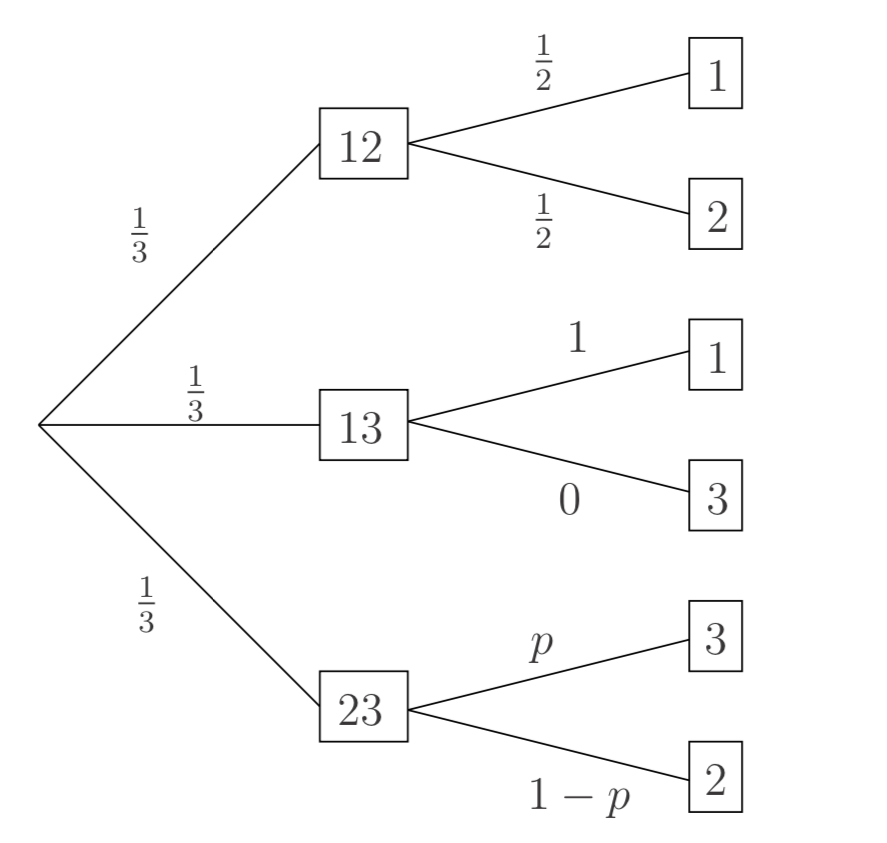
\includegraphics[width=100mm]{level1DT.png}
	\end{center}
	\caption{Schema of decision tree function}
	\label{Decision tree level 1}
\end{figure}
\\
\textbf{Level 2 decision tree}\\
Let us now go back to just three products, and assume that the consumer does not stop at one level of comparison,
but takes the winner of the first comparison and compares it with the remaining product. In this case
we have the level 2 decision tree shown in Fig. 13. Note that for the second comparison there is no
choice of products to compare, since there is only one product remaining. The probabilities of choosing each product are now\\
\begin{equation} \label{eq:14}
\begin{array}{l@{}l}
p_1 = \frac{1}{6}+\frac{1}{6}+\frac{p}{3}+\frac{1-p}{6}=\frac{1}{2}+\frac{p}{6} \\
p_2 = \frac{1-p}{6}+\frac{1}{6}+\frac{1-p}{6}=\frac{1}{2}-\frac{p}{3} \\
p_3 = \frac{p}{3}
\end{array}
\end{equation}
\\
Thus in this case the market share of product 1 does increase, so that there is a decoy effect.
Note, however, that the market share of the decoy product number 3, is the same as the increased market share of product 1.
\\
\begin{figure}[h!]
	\begin{center}
		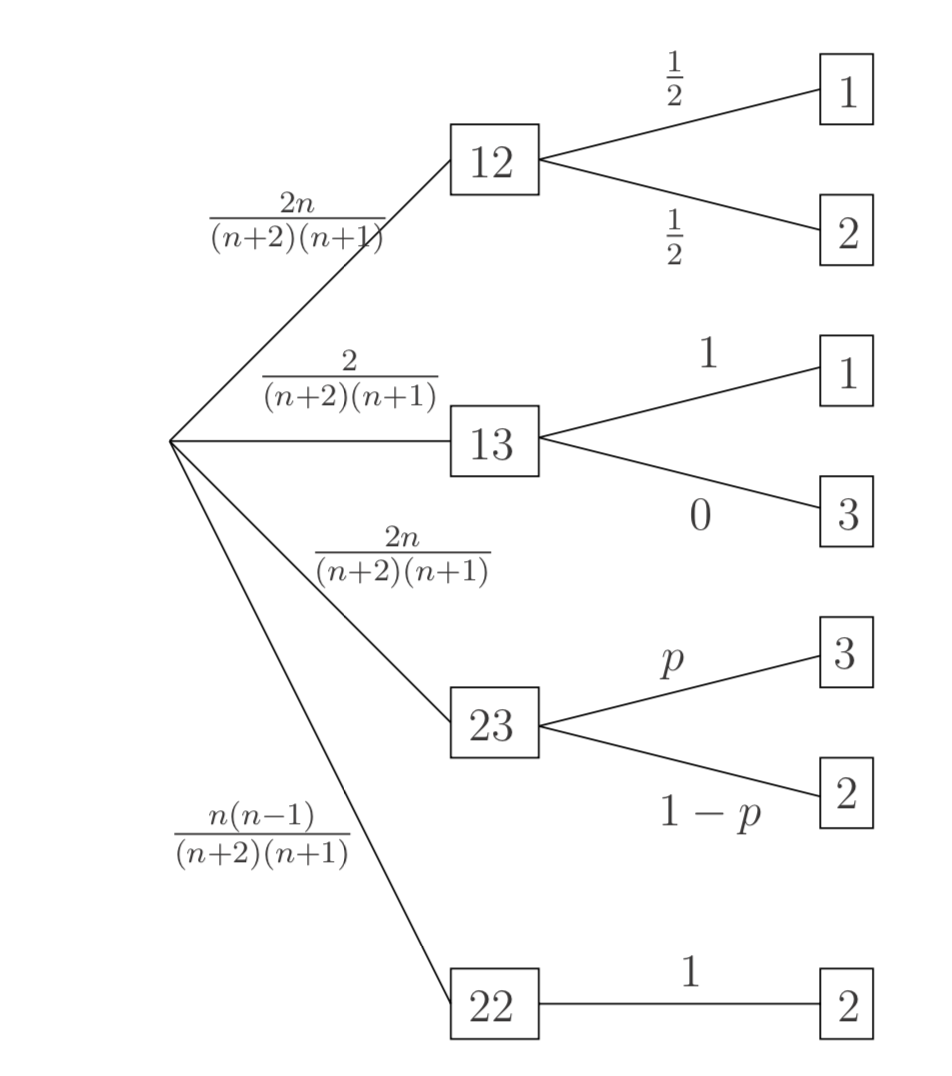
\includegraphics[height=100mm]{level2DT.png}
	\end{center}
	\caption{Basic schema of decision tree level 2}
	\label{Decision tree level 2}
\end{figure}
\newpage
\subsection{Propagation thrue a network} \label{subsec:propagation}
We consider here a simple linear model. Each node (I,J) is given, as psychology, a sensibility κkIJ to each quality k.
Each node, as loyalty, is influenced by the preceding nodes through a coefficient λIJ.
We have taken the interaction between the nodes so that (I, J) is affected only by its two immediate neighbours,
(I − 1, J) and (I, J − 1), and both exert the same influence per individual (the area of influence is easy to generalize).
In our simulations, the coefficients κkIJ and λIJ are positive and randomly chosen from a uniform distribution.
Consumer (I,J) forms an opinion or view, in the form of a composite numerical value, on product i according to
$$V_{IJ}^{i} = \sum_k K_{IJ}^kQ_{ki} + \lambda_{IJ}(V_{I-1,J}^1+V_{I,J-1}^i), for I > 0, J > 0$$
\\
\textbf{Binary comparisons} \label{subsec:binary}\\
Suppose a customer chooses to compare product i with product $j$.
What is the probability that he will choose $i$ over $j$?
In the Logit model we would simply have
\\
\begin{equation} \label{eq:15}
p_i = C exp(V_i - P_i), p_j = C exp(V_j - P_j)
\end{equation}
\\
where $C$ is chosen so that $p_i + p_j = 1$.

\begin{figure}[h!]
	\begin{center}
		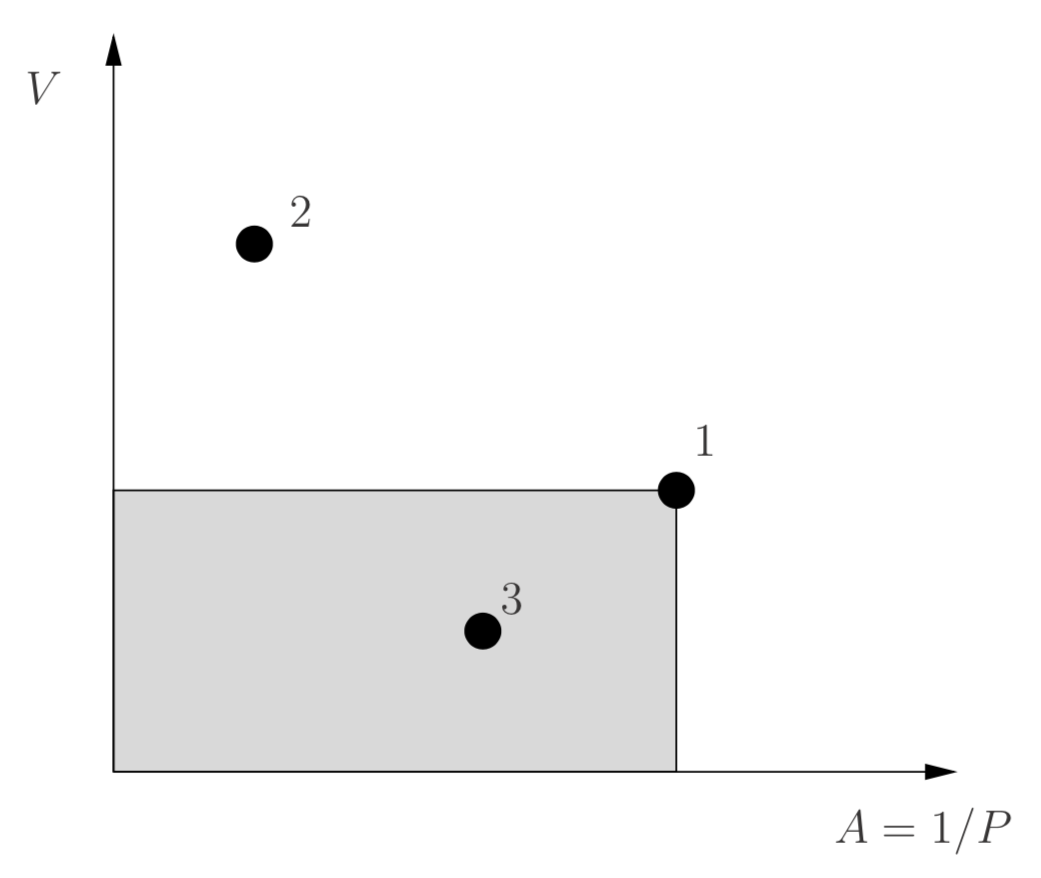
\includegraphics[width=100mm]{affordability.png}
	\end{center}
	\caption{Products in the affordability-value plane.
	The shaded region is the region of products dominated by product 1.}
	\label{Affordability of products}
\end{figure}

\section{A particle-dynamics model} \label{sec:dynamic}
The basic idea from~\cite{patel} is to build a model based on a physical analogy, between the customers buying behavior
and particle-particle dynamics.
We assume customers to be particles moving in quality space.
\begin{figure}[h!]
	\begin{center}
		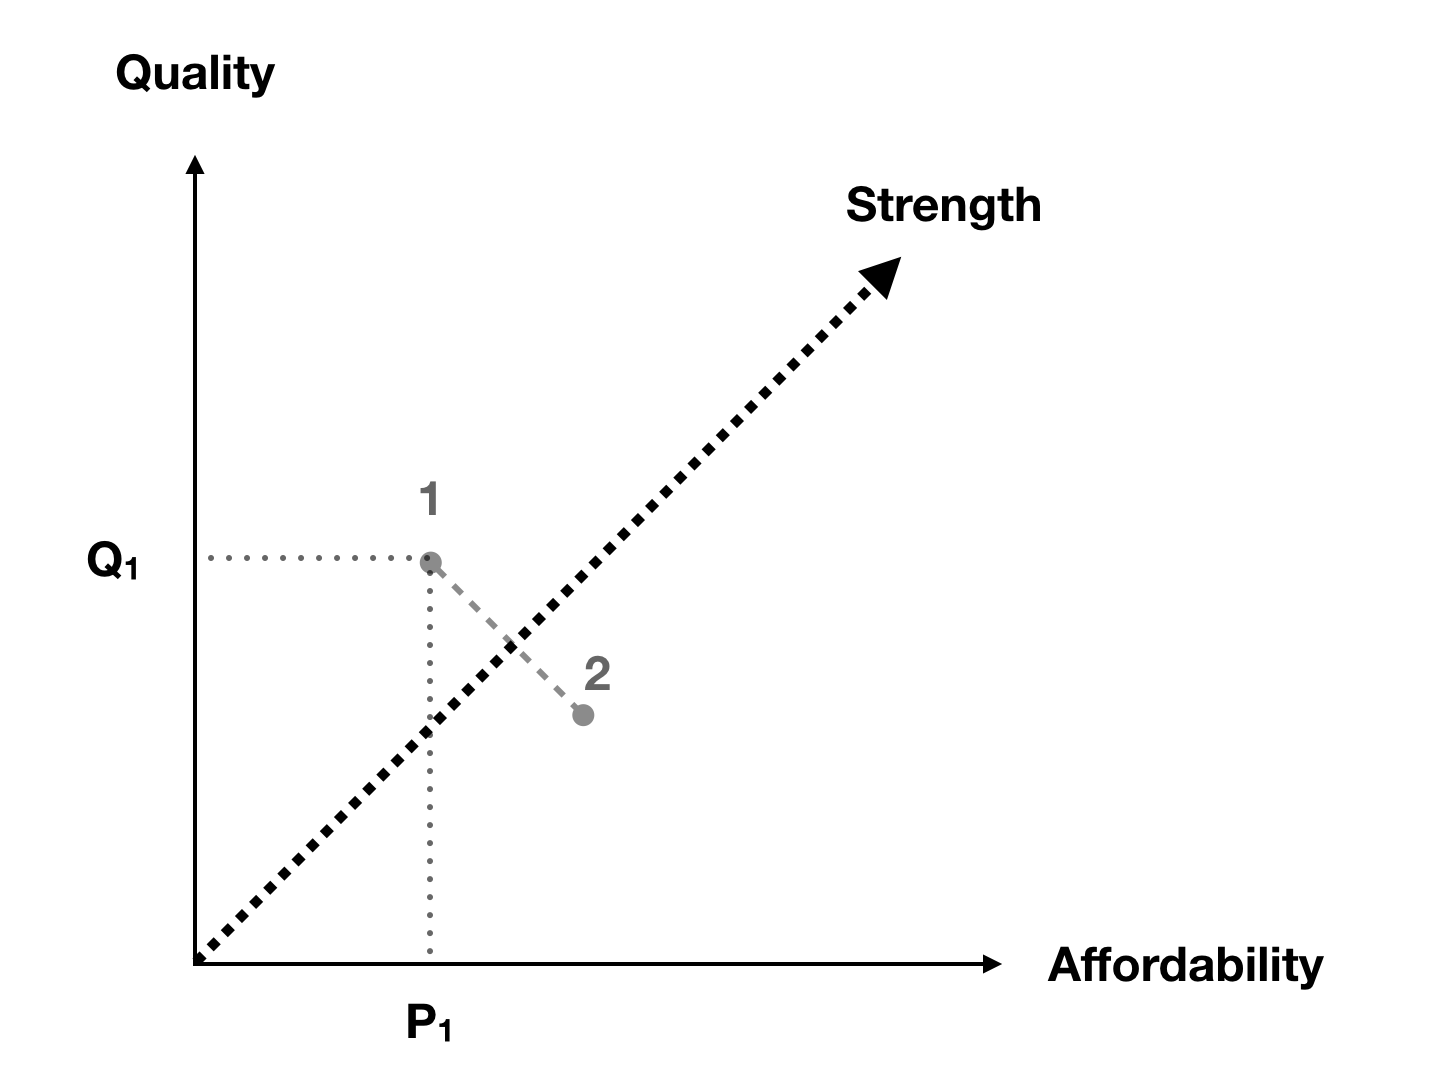
\includegraphics[width=80mm]{strength.png}
	\end{center}
	\caption{Product space with two products}
	\label{Strength of products}
\end{figure}
\\
The products are considered as sources of strength potentials, the details of the potentials depending on the products’ characteristics.
The psychology of people will be regarded as the influence of the potential on the mass of the particles.
This will depend on the customer but also on the characteristics of each product, weighted by coefficients of choice.
The sociology of individuals can be considered as a form of particle-particle interaction.
Following what has gone before, the product space is defined by just two characteristics for each product $i$ with affordability $P_i$ and quality $Q_i$.
We can define the ‘strength’ \footnote{ thw power if the product or service to be attractive for customer} of a product as the distance
of the product from the origin in product space as
\\
\begin{equation} \label{eq:16}
Ui = (Pi + Qi)/2
\end{equation}
\\
All the products with $Pi + Qi = constant$ will have the same strength.

\subsection{Dynamics of market share} \label{subsec:marketshare}
Market shares don't unusually depend in their qualitative behavior, on the coefficients $\alpha_{ij}$ and the values
of $\alpha_{ij}$ grow up as fast as their tend towards stability values.
In the situation  that $\alpha_{ij} \geq 0$ and $\alpha_{ij} + \alpha_{ji} > 0$ for $i \neq j$ the linear system looks like
\\
\begin{equation} \label{eq:17}
\frac{dX_i}{dt} = \sum_ja_{ij}X_j
\end{equation}
\\
where $a_{ij} = \alpha_{ij}$ for $i \neq j$ and $a_{ii} - \sum_{i \neq j}\alpha_{ji}$ turns out to have semi-definite
coefficient matrix.

\section{Statistic solutions of data prediction} \label{sec:statistics}
As a reference method for model result compare will be used time series prediction.
Time series data often arise when monitoring industrial processes or tracking corporate business metrics.
The essential difference between modeling data via time series methods or using the process monitoring methods.
Time series analysis accounts for the fact that data points taken over time may have an internal structure such as autocorrelation,
trend or seasonal variation that should be accounted for.\\
\\
\textbf{Analyze of time series} \label{subsec:statistics_analyze}\\
As is written by~\cite{benkova} we can divide time series to
\begin{itemize}
	\item subjective and objective
	\item quantitative, qualitative and causal
\end{itemize}\\
\\
\textbf{As basic characteristics we can define:}
\begin{itemize}
	\item absolute growth (1.difference)
	\begin{equation} \label{eq:18}
	\Delta_t^1 = y_t - y_{t-1}, t = 2,3 ....,n
	\end{equation}
	\item relative growth
	\begin{equation} \label{eq:19}
	\delta_1 = \frac{\Delta_t^1}{\Delta_{t-1}^1}, t = 2,3 ....,n
	\end{equation}
	\item growth coefficient
	\begin{equation} \label{eq:20}
	k_t = \frac{y_t}{y_{t-1}}, t = 2,3 ....,n
	\end{equation}
\end{itemize}\\
\\
Modeling of time series can be done by one-dimensional or two-dimensional models.
Basic one-dimensional model is used in situation where expected that time will be the only one variable.\\
\\
\textbf{Classical model of time series have these components:}
\begin{itemize}
	\item $T_t$ trends component, characteristic of long term trend
	\item $C_t$ cyclical component, fluctuation around trend
	\item $S_t$ seasonal component, periodical component repeated in time
	\item $I_t$ irregular component, random component, stay in time series after all corrections
\end{itemize}
\\
For pur need we will be used only Linear $T_t = a_0 = \overset{-}{y}, t = 1,2, ...., n$ and exponential trend
$T_t = a_{0}a_1^t, t = 1,2,....,n, a_1 > 0$.
\\
For testing which model is better for our test scenario we use Fisher test \footnote{Fisher's exact test is a statistical test
used to determine if there are nonrandom associations between two categorical variables.
For each one, calculate the associated conditional probability using, where the sum of these probabilities must be 1.} of local extrema
in periodogram and Durbin Watson test \footnote{The Durbin Watson statistic is a test for autocorrelation in the residuals
from a statistical regression analysis.
The Durbin-Watson statistic will always have a value between 0 and 4.
A value of 2.0 means that there is no autocorrelation detected in the sample.} of autocorrelation.\\
\\
\textbf{Forecasting with Single Exponential Smoothing} \label{subsec:statistics_forecast}
\\
The forecasting formula is the basic equation
\begin{equation} \label{eq:21}
S_t+1 = \alpha y_t+(1−\alpha)S_t, 0< \alpha \leq 1,t>0
\end{equation}
\\
This can be written as:
\begin{equation} \label{eq:22}
S_t+1=S_t+\alpha \epsilon_t
\end{equation}
\\
where $\epsilon_t$ is the forecast error (actual - forecast) for period $t$.
In other words, the new forecast is the old one plus an adjustment for the error that occurred in the last forecast.\\
\\
\textbf{Bootstrapping of Forecasts}\\
If you wish to forecast from some origin, usually the last data point, and no actual observations are available
we have to modify the formula to become:
\\
\begin{equation} \label{eq:23}
S_t+1 = \alpha y_{org}+(1−\alpha)S_t
\end{equation}
\\
where $y_{orig}$ remains constant.
